%\subsection{Effect of Attention Width}
%Our model has a parameter $K$ that specifies the number of entities to attend to. 
We investigated the effect of the multi-focus attention beam size $K$ by evaluating performance
on the CoNLL test-a dataset for different values of $K$. Results 
are shown in \figref{fig:k_effect}. It can be seen that performance peaks at $K=3$, with a sharp decrease after $K=10$. 

\comment{
\begin{figure}[t!]
\includegraphics[width=\linewidth]{./k_effect.png}
\caption{Effect of parameter $K$ on entity linking accuracy. Results shown for the testa Conll dataset, where the model
is trained on Conll training data. }
\label{fig:k_effect}
\end{figure}
}
% PGF plot version of the figure
{
\pgfplotsset{every tick label/.append style={font=\tiny}}
\begin{figure}
\centering
\resizebox {\columnwidth} {!} {
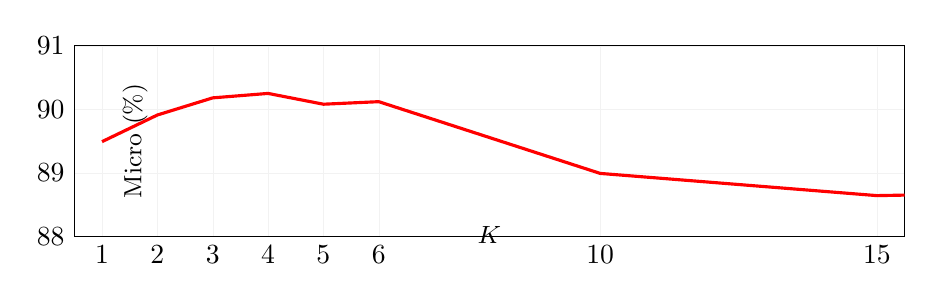
\begin{tikzpicture}
  \begin{axis}[
   %title  = Effect of K,
   width = \columnwidth,
   height=4cm,
%    ybar,
 %   bar width = 0.2cm,
    %x axis line style = { opacity = 0 },
    %axis y line       = none,
    tickwidth         = 0pt,
    xmin=0.5,xmax=15.5,
    ymin=88,ymax=91,
    grid=both,
    grid style={line width=.1pt, draw=gray!10},
    x label style={at={(axis description cs:0.5,0.1)},anchor=north},
    y label style={at={(axis description cs:0.1,.5)},anchor=south},
    xlabel={\small $K$},
    ylabel={\small Micro (\%)},
   % enlarge y limits  = 0.2,
    xtick = data,
  ]
  \addplot [line width=0.4mm, red] coordinates { 
    (1,89.49) (2,89.91)  (3,90.18) (4,90.25) (5,90.08) (6,90.12) (10,88.99) (15,88.64) (20,88.72)
  };
  \pgfresetboundingbox
  %\addplot coordinates { (20,1)         (15,2)
   %                      (60,3)   (75,4)  };
 % \legend{Topics, Posts}
  \end{axis}
\end{tikzpicture}
}
\caption{Effect of parameter $K$ on entity linking accuracy. Results shown for the testa Conll dataset, where the model
is trained on Conll training data. }
\end{figure}
}

%(1,89.72) (2, 89.77) (3, 90.39) (4, 90.39) (5, 90.52)   (6,90) (7,90) (8,90) (9,90) (10,90)   (11,90) (12,90) (13,90) (14,90) (15,90)};